\documentclass[12pt]{article}%
\usepackage{amsfonts}
\usepackage{fancyhdr}
\usepackage{comment}
\usepackage[a4paper, top=2.5cm, bottom=2.5cm, left=2.2cm, right=2.2cm]%
{geometry}
\usepackage{times}
\usepackage{amsmath}
\usepackage{changepage}
\usepackage{amssymb}
\usepackage{graphicx}%
\usepackage{float}
\usepackage{subfigure}
\usepackage{xcolor}
\setcounter{MaxMatrixCols}{30}
\newtheorem{theorem}{Theorem}
\newtheorem{acknowledgement}[theorem]{Acknowledgement}
\newtheorem{algorithm}[theorem]{Algorithm}
\newtheorem{axiom}{Axiom}
\newtheorem{case}[theorem]{Case}
\newtheorem{claim}[theorem]{Claim}
\newtheorem{conclusion}[theorem]{Conclusion}
\newtheorem{condition}[theorem]{Condition}
\newtheorem{conjecture}[theorem]{Conjecture}
\newtheorem{corollary}[theorem]{Corollary}
\newtheorem{criterion}[theorem]{Criterion}
\newtheorem{definition}[theorem]{Definition}
\newtheorem{example}[theorem]{Example}
\newtheorem{exercise}[theorem]{Exercise}
\newtheorem{lemma}[theorem]{Lemma}
\newtheorem{notation}[theorem]{Notation}
\newtheorem{problem}[theorem]{Problem}
\newtheorem{proposition}[theorem]{Proposition}
\newtheorem{remark}[theorem]{Remark}
\newtheorem{solution}[theorem]{Solution}
\newtheorem{summary}[theorem]{Summary}
\newenvironment{proof}[1][Proof]{\textbf{#1.} }{\ \rule{0.5em}{0.5em}}

\newcommand{\Q}{\mathbb{Q}}
\newcommand{\R}{\mathbb{R}}
\newcommand{\C}{\mathbb{C}}
\newcommand{\Z}{\mathbb{Z}}

\begin{document}

\noindent \today


\section{Introduction}



%!TEX root = Main.tex

\section{Model} %%% introcude $Gamma_a, a=1,\cdots,k$ somewhere in this section!
% \subsection{Notations}


\subsection{Stochastic block model} % deleted the "undirected" setting
A set of $n$ nodes $\Gamma=\left\{ v_1,\cdots,v_n \right\}$ is partitioned into $k$ clusters $\Gamma_1,\cdots,\Gamma_k$. For simplicity, we use the notation $i\in\Gamma_l$ to denote that $v_i\in\Gamma_l$. The cluster of node $v_i$ is represented by $z_i\in \left\{ 1,\cdots,k \right\}$, and the vector of clusters is $\bz=\left( z_i \right)_{i=1}^n $. 
Define the adjacency matrix $\bA\in \left\{ 0,1\right\}^{n\times n}$ where  $\bA_{i,j}= 1$ if an edge is observed between $v_i$ and $v_j$ and $\bA_{i,j}=0$ otherwise.
We set $\mathbf{A}_{i,i}\equiv 0$  for any $i=1,\cdots,n$, 
and assume that $\bA_{i,j}$'s are conditionally independent given the cluster vector $\bz$:
\begin{align*}
\mathbf{A}_{i,j}|z_i=q,z_j=l \overset{ind}{\sim} \text{Bernoulli}(\mathbf{C}_{q,l}), \qquad i\neq j,
\end{align*}
where $\mathbf{C}\in [0,1]^{k\times k}$ denote the  connecting probability matrix.



\subsection{Dynamic generalization of the stochastic block model}
Consider a growing dynamic network where edges appear over time. 
Assume that the edges will not disappear once constructed,
and that the observed point processes ${N}_{i,j}(\cdot)\in \left\{ 0,1 \right\}$ are independent realizations of intensity functions 
\begin{align*}
\lambda_{i,j}(t)=f_{z_i,z_j}(t-\tau_{i,j})\cdot g(d_{i,j}), \qquad t\in[0,T],\quad i,j=1,\cdots,n, 
\end{align*}
where $[0,T]$ is overall time period,
$\tau_{i,j}$ is the time lag of the edge from $v_i$ to $v_j$, 
 $d_{i,j}$ is the spatial distance between $v_i$ and $v_j$, $f_{z_i,z_j}(\cdot)$ is the connecting intensity function from cluster $z_i$ to $z_j$, and $g(\cdot)$ is a decreasing function that accounts for the decay of connection as the distance between any pair of nodes increases.
Similar to the stochastic block model, we set $\lambda_{i,i}(\cdot)\equiv 0$ for $i=1,\cdots,n$.
% Add more rigorous definition of point process and intensity function.
\\
The integrated point process $N_{i,\cdot}(\cdot):=\sum_{j\neq i} N_{i,j}(\cdot)$ can be viewed as a realization of the intensity function $\lambda_{i,\cdot}(\cdot)=\sum_{j\neq i}\lambda_{i,j}(\cdot)$.
For convenience, we denote $N_{i,\cdot}(\cdot)$ by $N_i(\cdot)$, and $\lambda_{i,\cdot}(\cdot)$ by $\lambda_{N_i}(\cdot)$. 

In many applications, the edge from $v_i$ to $v_j$ is determined only by the activity of $v_i$. 
So we may have the following assumption.
\begin{assumption}\label{asp:time lag}
$\tau_{i,j}$ only depends on $v_i$, that is,
$\tau_{i,j}=\tau_i $ for all $j\neq i, i=1,\cdots,n$.
\end{assumption}
\noindent With Assumption \ref{asp:time lag}, $\lambda_{N_i}(\cdot)$ can be written as
\begin{align*}
\lambda_{N_i}(t) &= \sum_{l=1}^k \left( f_{z_i,l}(t-\tau_i)\cdot \sum_{j\in\Gamma_l,j\neq i}g(d_{i,j}) \right) \\
&=: \sum_{l=1}^k  f_{z_i,l}(t-\tau_i)\cdot w_{i,l}.
\end{align*}
Here $w_{i,l}$ measures the overall distance between node $v_i$ and cluster $\Gamma_l$. 
For example, if the nodes represent neurons and are clustered by cell types, $w_{i,l}$ represents the distance between $v_i$ and its neighbor cells  which belong to cell types $l$.
We assume that the cell types are distributed uniformly in the sense that $w_{i,l}$ and $w_{j,l}$ are identically distributed for any $i, j$ such that $z_i=z_j$.
More formally, we have the following assumption.
 % which means $w_{i,l}=\bar w_{z_i,l}+\epsilon_{i,l}$ where $\left\{ \epsilon_{i,l} \right\}_{i\in\Gamma_l}$ are i.i.d. random variables with mean zero.

\begin{assumption}\label{asp:same distr}
$w_{i,l}=\bar w_{z_i,l}+\epsilon_{i,l}$ where $\left\{ \epsilon_{i,l} \right\}_{i\in\Gamma_l,l=1,\cdots,k}$ are i.i.d. random variables with mean $0$ and variance $\sigma^2<\infty$.
\end{assumption}
\noindent
By Assumption \ref{asp:time lag} and \ref{asp:same distr}, $\lambda_{N_i}(t)=\lambda_{z_i}(t-\tau_i)+\sum_{l=1}^kf_{z_i,l}(t-\tau_i)\epsilon_{i,l}$ for $t\in[0,T]$, where $\lambda_{z_i}(t):=\sum_{k=1}^lf_{z_i,l}(t)\cdot\bar w_{z_i,l}$.

\subsubsection*{Minor comments}
Hoeffding's inequality might be useful later. (If $\epsilon_{1},\cdots,\epsilon_d\overset{i.i.d}{\sim}\text{sub-G}(\tau_0)$ and $\mathbb{E}\epsilon_{i}=0$, then $\mathbb{P}(\langle a,\epsilon\rangle\geq t)\leq \exp \left\{ -t^2/(2\|a\|_2^2\tau_0^2) \right\}$ for any $a\in \mathbb{R}^d$.)

Let $\mathbf{F}_{k\times k} = [f_{q,l}(\cdot)]_{q,l\in \left\{ 1,\cdots,k \right\}}$, $\mathbf W_{n\times k} = [w_{i,l}]_{i\in \left\{ 1,\cdots,n \right\}, l\in \left\{ 1,\cdots,k \right\}}$, $\mathbf{Z}\in \left\{ 0,1 \right\}^{n\times k}$ with $\mathbf Z_{i,l}=1$ if $z_i=l$ and $0$ otherwise. Then
\begin{align*}
\begin{bmatrix}
\lambda_{N_1}(\cdot+\tau_1)\\
\vdots\\
\lambda_{N_n}(\cdot+\tau_n)
\end{bmatrix}=\text{diag}\left( \mathbf{ZFW}^\top \right) .
\end{align*}



\section{Method}
\section{Theory}

%!TEX root = Main.tex

\section{Simulation}

We analyze the network with two types of nodes.
The first type of nodes (type I) are equispaced points on $x=1$ and $0\leq y\leq 6$.
The second type of nodes (type II) are generated uniformly in $[0,2]\times[0,6]$. 
Figure \ref{fig: nodes} gives an example of 30 nodes, among which 3 are from type I and the rest 27 are from type II.
\\
\begin{figure}[H]
\centering
\includegraphics[width=0.5\textwidth]{../simulation/nodes_distribution}
\caption{30 nodes with three belonging to group 1.}
\label{fig: nodes}
\end{figure}

Some edges are constructed between pairs of nodes during time period $[0,50]$.
Nodes are connected if and only if there distance is less than $1.5$.
For the nodes of the same type, the connecting time is generated from uniform distribution $U(0,40)$.
For the pair of nodes with one from type I and the other from type II, the connecting time is distributed as $N(5+\tau,1)$, where $\tau$ is the time delay caused by the type I node and is generated randomly from $U(0,30)$.

The case with 3 type I nodes and 27 type II nodes is tested.
Clustering error rate is recorded for 10 independent trials. 
Due to the uncertainty caused by initialization, five independent initializations are used for each trial, and only the one with the largest distance between estimated mean curves is kept.
The average error rate is $1.3/30=4.3\%$.



% To show the development of the network, we plot snapshots in Fig.\ref{Fig: development of network} of the network $\mathbf{G}_1$  at time points $t=0.01, 0.1, 1, 10, 100$.
% \begin{figure}
% \centering
% 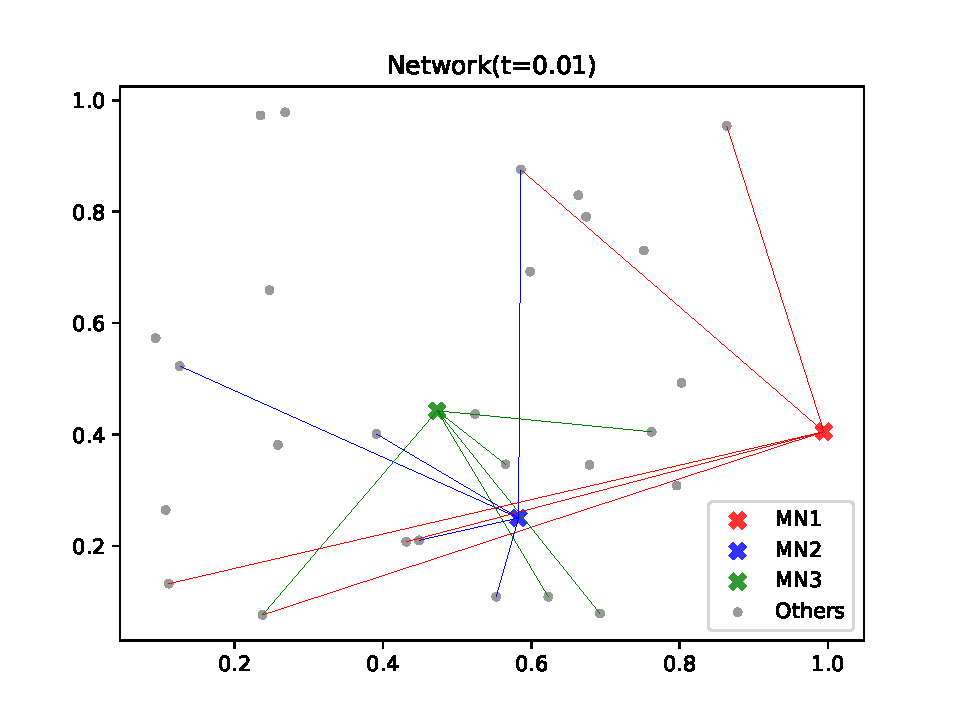
\includegraphics[width = 0.3\textwidth]{Graphs/t_001.pdf}
% 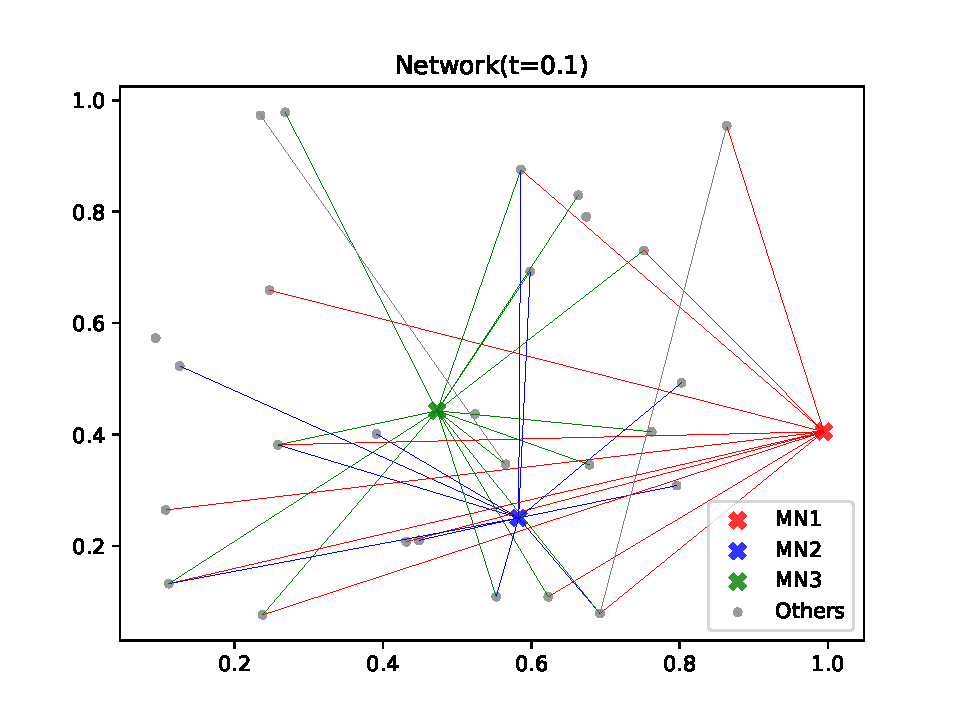
\includegraphics[width = 0.3\textwidth]{Graphs/t_01.pdf}
% 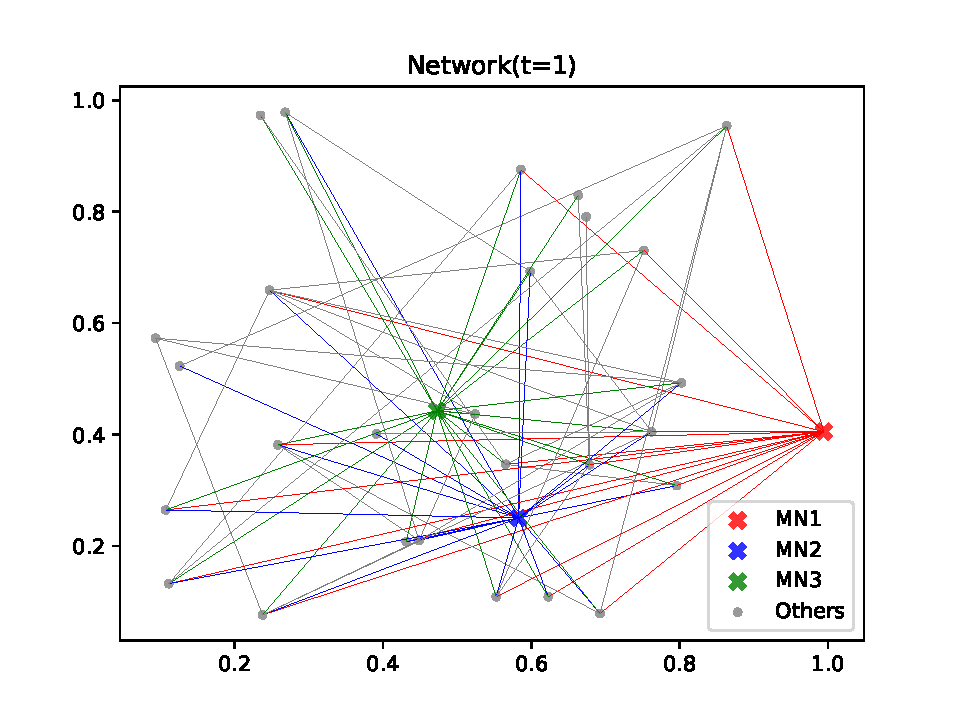
\includegraphics[width = 0.3\textwidth]{Graphs/t_1.pdf}\\
% 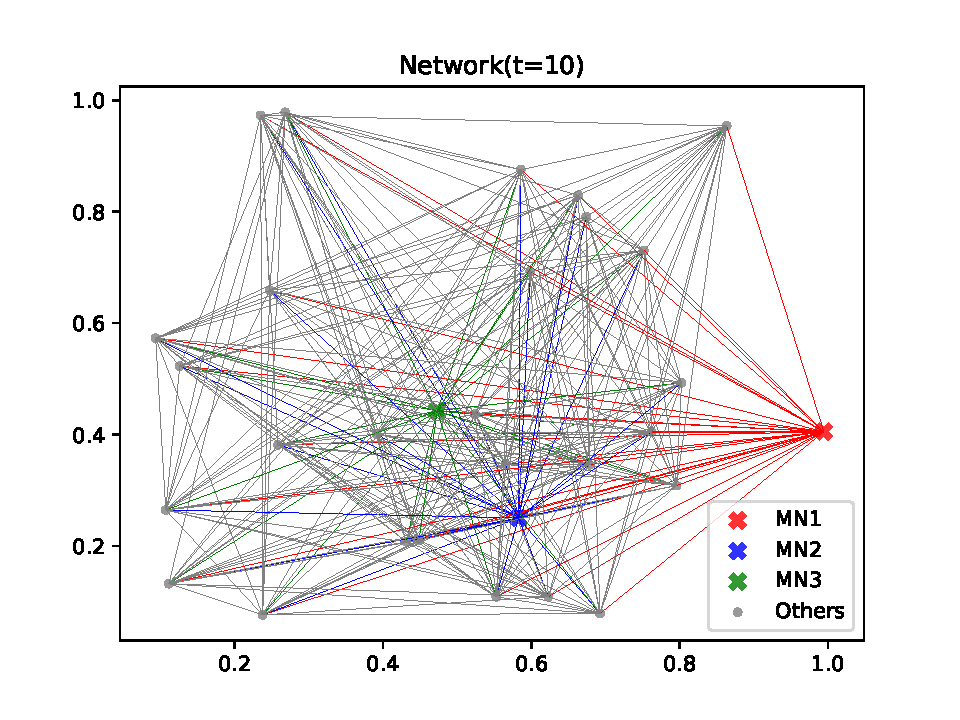
\includegraphics[width = 0.3\textwidth]{Graphs/t_10.pdf}
% 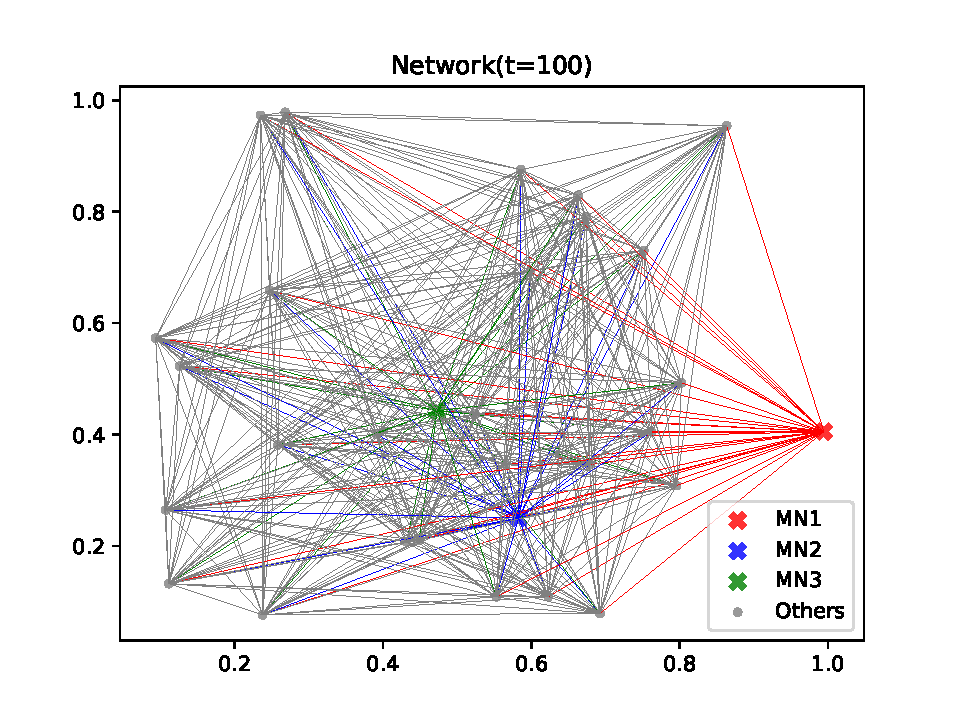
\includegraphics[width = 0.3\textwidth]{Graphs/t_100.pdf}
% \caption{Development of the network with two cell types. The node $n_1$ is represented by ``MN1'' in red. The node $n_2$ is represented by ``MN2'' in blue. The node $n_3$ is represented by ``MN3'' in green. Other nodes are represented by ``Others'' in gray.}
% \label{Fig: development of network}
% \end{figure}





\bibliographystyle{abbrv}
\bibliography{/Users/bgemily/Documents/Academic/SC/graphon}












\end{document}